\documentclass[11pt,twoside]{book}

\usepackage{geometry}
\geometry{papersize={150mm,200mm}}
\geometry{tmargin=1cm,bmargin=1cm,lmargin=1cm,rmargin=1cm}

\usepackage{xcolor}
\usepackage{bm}
\usepackage[e]{esvect}

\usepackage{tikz}
%%\usepackage{tikz-3dplot} % needs tikz-3dplot.sty in same folder
\usetikzlibrary{calc}
\usetikzlibrary{angles, quotes}
\usetikzlibrary{arrows, arrows.meta}

\usepackage{xintexpr}

\makeatletter
\newcommand*\dotp{\mathpalette\dotp@{.5}}
\newcommand*\dotp@[2]{\mathbin{\vcenter{\hbox{\scalebox{#2}{$\m@th#1\bullet$}}}}}
\makeatother
\newcommand\dotdotp{\dotp\hspace{-0.16em}\dotp\hspace{0.20em}}

\makeatletter
\newcommand{\raisemath}[1]{\mathpalette{\raisem@th{#1}}}
\newcommand{\raisem@th}[3]{\raisebox{#1}{$#2#3$}}
\makeatother

\usepackage{nicefrac}

\usepackage{gensymb} % for \degree

\usepackage{verbatim}

\usepackage[english]{babel}
\addto\captionsenglish{\renewcommand{\figurename}{figure}}
\addto\captionsenglish{\def\figureshortname{fig.}}
\newcommand\figref[1]{\figureshortname~\ref{#1}}

\usepackage[format=plain]{caption}
\captionsetup[figure]{%
font={small,it},labelfont=small,%
labelsep=newline,justification=centering,singlelinecheck=off,%
aboveskip=4mm,belowskip=2.5mm}

\newcommand{\lquote}[0]{``}
\newcommand{\rquote}[0]{''}
\newcommand{\inquotes}[1]{\lquote{#1}\rquote}

\pagestyle{empty}

\begin{document}

\begin{center}

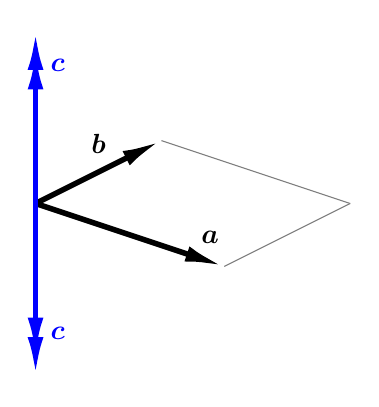
\begin{tikzpicture}[scale=0.999]
	\draw [line width=2pt, black, -{Latex[length=5mm, width=2mm]}]
		(0,0) -- (2.4,-0.8)
		node[above=1.4mm, xshift=-1.8mm] {$\bm{a}$};
	\draw [line width=2pt, black, -{Latex[length=5mm, width=2mm]}]
		(0,0) -- (1.6,0.8)
		node[midway, above=0.8mm] {$\bm{b}$};
	\draw [line width=2pt,blue,-{Latex[length=5mm, width=2mm]}]
		(0,0) -- (0,-1.95);
	\draw [line width=2pt,blue,-{Latex[length=5mm, width=2mm]}]
		(0,0) -- (0,-2.2)
		node[pos=0.75, right, xshift=0.4mm] {$\bm{c}$};
	\draw [line width=2pt,blue,-{Latex[length=5mm, width=2mm]}]
		(0,0) -- (0,1.95);
	\draw [line width=2pt,blue,-{Latex[length=5mm, width=2mm]}]
		(0,0) -- (0,2.2)
		node[pos=0.8, right, xshift=0.4mm] {$\bm{c}$};
	\draw [line width=0.4pt, black!50] (2.4, -0.8) -- (4, 0);
	\draw [line width=0.4pt, black!50] (1.6, 0.8) -- (4, 0);
\end{tikzpicture}

\end{center}

\end{document}
